%! Author = melek
%! Date = 22.01.2023

% Preamble
\documentclass[11pt]{article}

% Packages
\usepackage{amsmath}
\usepackage{graphicx}
\graphicspath{ {../images/} }

\title{Assignment 3: Q-Learning and Actor-Critic Algorithms}
\author{huseyinabanox@gmail.com}
\date{January 2023}

% Document
\begin{document}

    \maketitle

    \section{Part 1: Q-Learning}

    \subsection*{Question 1: basic Q-learning performance (DQN)}

    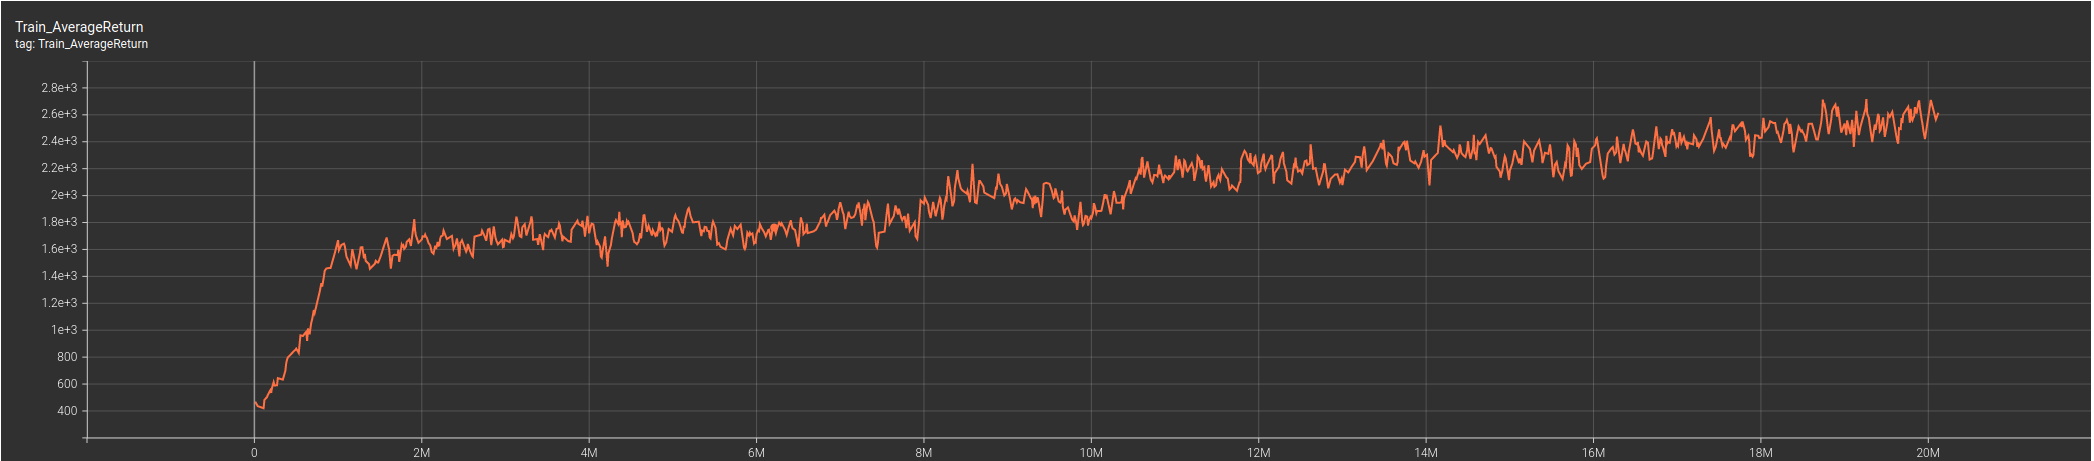
\includegraphics[scale=0.8]{q1/packman-20M}

    After 20M iterations the learning curve looks like above.
    Relevant log files can be found under data folder.

    The reference Pac-Man implementation for 1 million steps gets a return of 1500 in this timeframe.
    Our solution also gets the same returns.
    After 20M steps the return reaches to 2800 and keeps the positive trend.
    The test is conducted on a CPU machine for 2 days and interrupted early on.
    If it were let to continue the results are expected to improve.

    \subsection*{Question 2: double Q-learning (DDQN)}

    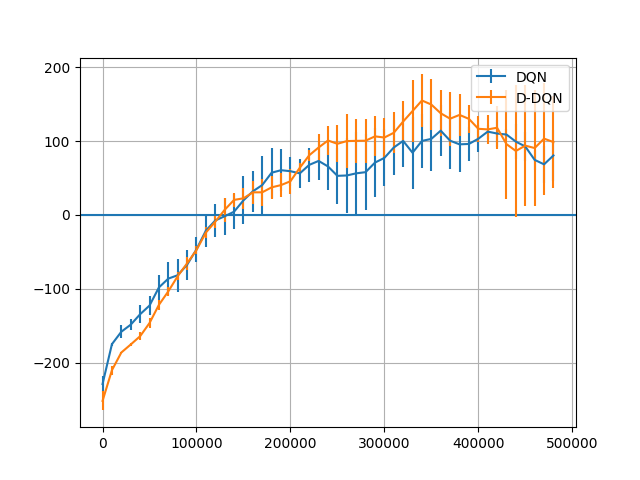
\includegraphics[scale=0.8]{q2/q2}

    LunarLander-v3 environment is used for 3 seeds per configuration e.g. DQN vs D-DQN as stated in the question.
    Different seed results are averaged and the plot above is generated.
    combine\_results\_q2.py file is used to combine results.

    Double Q network obtains better returns, as expected.
    the double estimator improves the accuracy of the learned Q values.

    Just like the reference solution with the default hyperparameters, our solution achieves around 150 reward after 350k timesteps, but there is considerable  variation between runs and without the double-Q trick the average return often decreases after reaching 150.

    \subsection*{Question 3: experimenting with hyperparameters}

    Three different hyper-parameters are selected and a different value is selected to test the impact on the accuracy of the model.
    The test is conducted on Lander environment.
    This test is actually an extension of the question 2 with different parameters and just the vanilla dqn is used.


    First learning rate is multiplied by 10.
    Increasing the learning rate may speed up learning.
    In our case the results worsen which means the selected learning rate is too big.
    Another test may be run using half of the selected learning rate.
    The results are shown in the first column of the image.

    In the second test exploration schedule is changed.
    The exploration rate is started as 1 as in the default case.
    It is decreased gradually to 0.01 over the half of the total steps and kept constant.
    In this setting the training is expected to explore more and the returns are expected to improve.
    However the accuracy worsens.
    Maybe because the exploration rate is not enough.
    Another test may be run using the default minimum exploration rate 0.2 for half the steps or more to see affect of more exploration.
    The results are shown in the second column of the image.

    In the second test number of layers decreased from 3 to 2, hence no hidden layer is used.
    In this setting the returns reaches 150 without double dqn and keeps relatively stable.
    This indicates a 3 layer network in this setting is not best fit for the problem and simplifying the architecture helps to improve the returns.
    The results are shown in the third column of the image.

    \hspace*{-0.5in}
    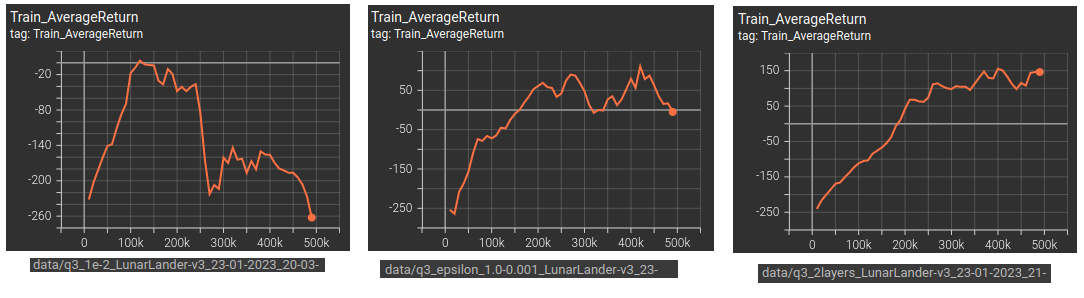
\includegraphics[scale=1.5]{q3/q3}

    \section{Part 2: Actor-Critic}

    \subsection*{Question 4: Sanity check with Cartpole}

    Actor critic algorithm is tested in cartpole environment.
    Different target update parameters and gradient steps parameters are tried.

    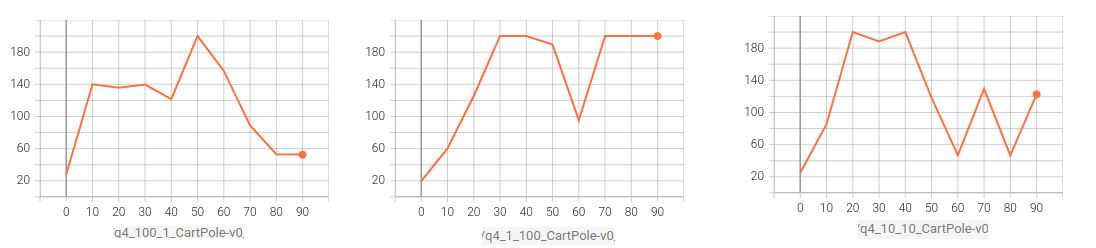
\includegraphics[scale=1.5]{q4/q4}.

    Subtitles show the used parameters.

    Best performance is obtained when both parameters are set to 10.
    If target update is set to 1 and gradient steps are set to 100, learning seems to be more stable.
    This results shows the importance of gradient steps.

    \subsection*{Question 5: Run actor-critic with more difficult tasks}

    Best results are obtained when both parameters are set to 10.

    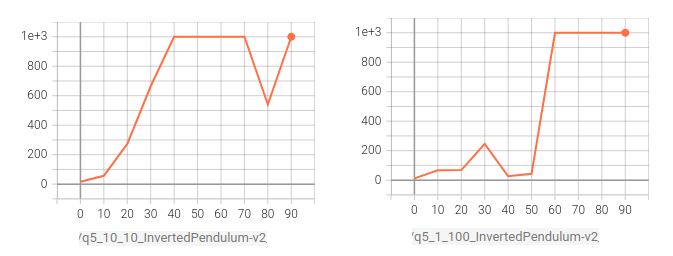
\includegraphics[scale=2]{q5/q5_inverted_pendulum}.

    After 100 iterations, InvertedPendulum return is around 1000, as expected.
    After 20 iterations, InvertedPendulum return should is above 100, as expected.

    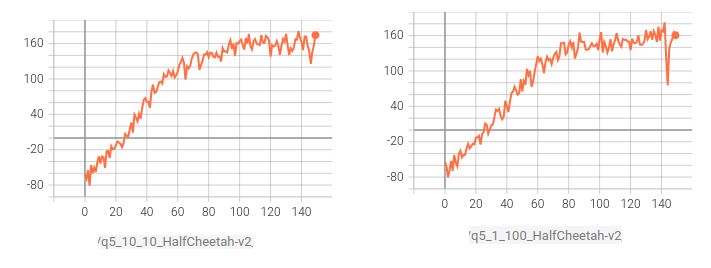
\includegraphics[scale=2]{q5/q5_half_cheetah}.

    After 150 iterations, HalfCheetah return is around 150, as expected.
    After 20 iterations, HalfCheetah return is above -40, as expected.

    \section{Part 3: Soft Actor-Critic}



    \subsection*{Question 6: Run soft actor-critic more difficult tasks}

    Actor updates and critic updates are set to 10.

    After 20000 steps, InvertedPendulum return is expected to reach 1000.
    Actually it is reached after 9k steps.

    \subsection*{Question 6: Run soft actor-critic more difficult tasks}

    The same parameters are used as stated in the question.
    Additionally \textless num\_critic\_updates\_pe\_agent\_update\textgreater and \textless num\_acto\_updates\_per\_agent\_update\textgreater parameters are set to 10.

    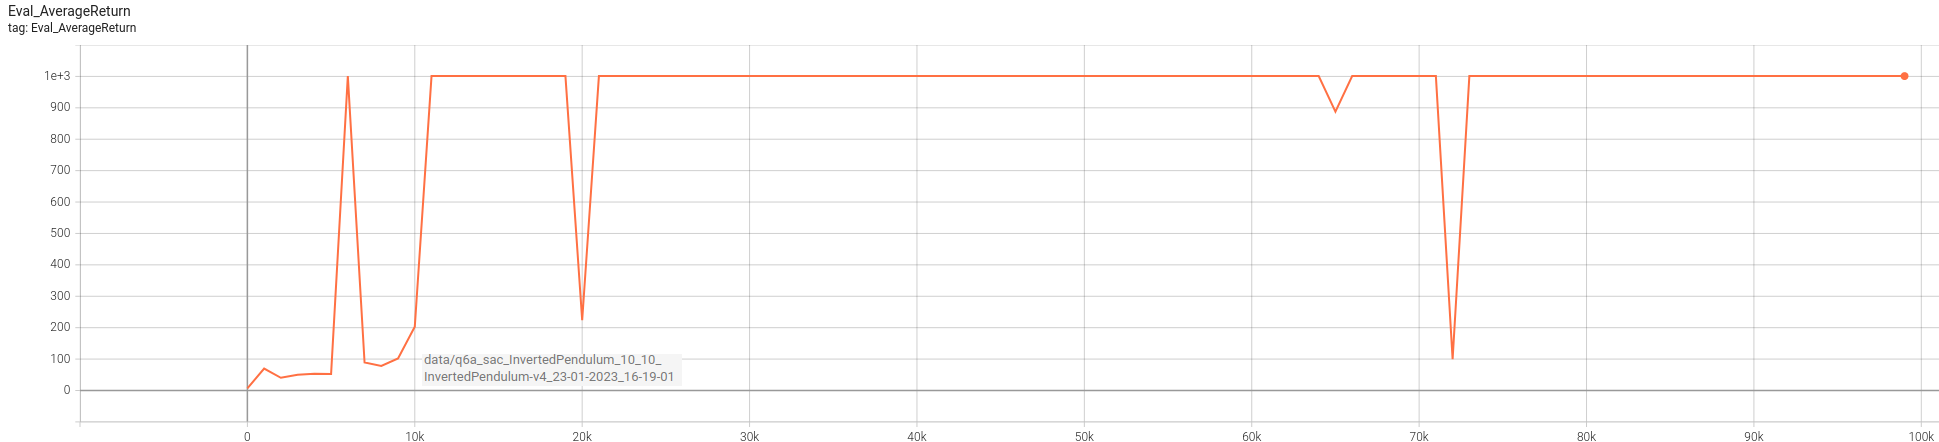
\includegraphics[scale=0.66]{q6/inverted_pendulum}.

    After 10000 steps, InvertedPendulum return is expected to be near or above 100.
    After 20000 steps, InvertedPendulum return is expected to reach 1000.
    Our implementation reaches 1000 before 10K steps and stabilizes around 1000 after 10K steps.

    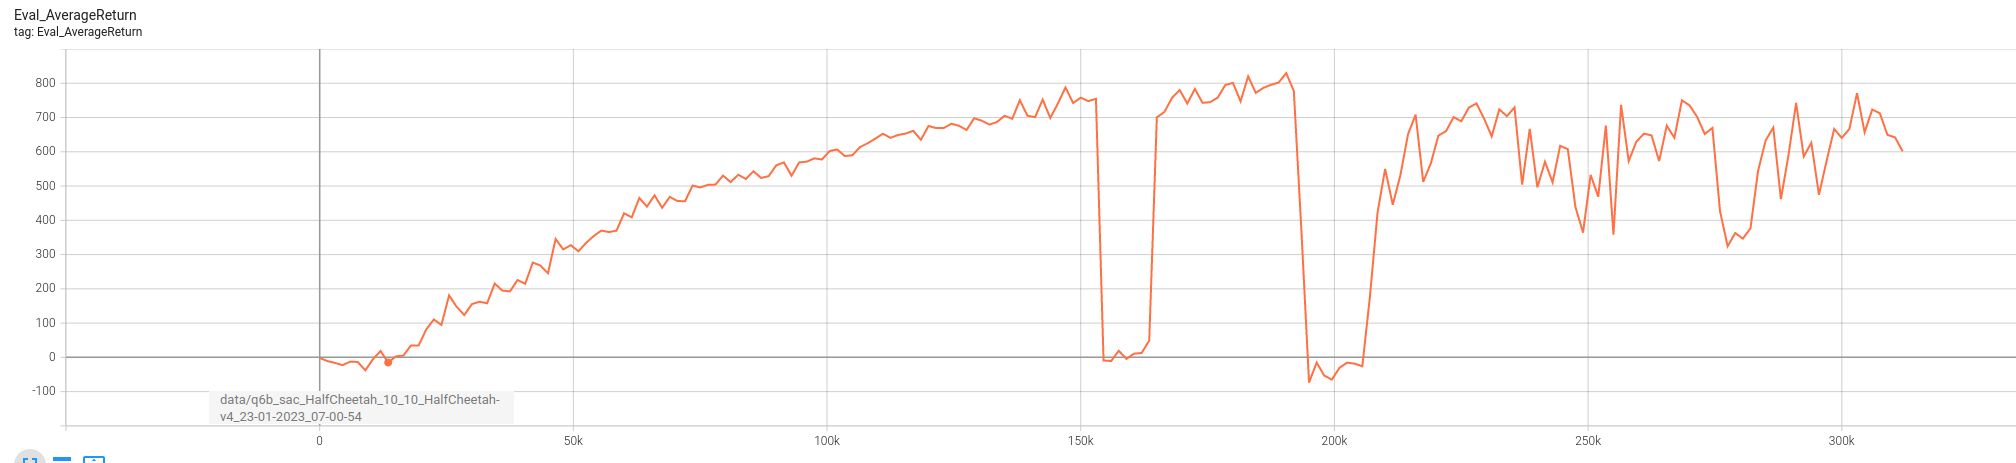
\includegraphics[scale=0.66]{q6/halfcheatah}.

    After 10000 steps, HalfCheetah return is expected to be above -40 (trending toward positive).
    After 50000 steps, HalfCheetah return should be around 200.
    Our implementation return is close to zero at 10K steps and is above 300 after 50K steps.




\end{document}